\documentclass{article}
\usepackage{graphicx}
\usepackage{natbib}
\usepackage{graphicx}
\bibliographystyle{plainnat}
\usepackage{fancyheadings}
\usepackage{tabularx}
\usepackage{alltt, parskip, boxedminipage}
\usepackage{makeidx, multirow, longtable, tocbibind, amssymb}
%\usepackage{fullpage}
\makeindex
\usepackage[usenames]{color}
\definecolor{darkblue}{rgb}{0,0.05,0.35}

\usepackage[dvips, pagebackref, pdftitle={}, pdfcreator={epydoc 2.1}, bookmarks=true, bookmarksopen=false, pdfpagemode=UseOutlines, colorlinks=true, linkcolor=black, anchorcolor=black, citecolor=black, filecolor=black, menucolor=black, pagecolor=black, urlcolor=darkblue]{hyperref}
\setlength{\textheight}{21.5cm}
\setlength{\textwidth}{18cm}
\setlength{\hoffset}{-3.0cm}
\setlength{\footskip}{1.5cm}
\setlength{\headsep}{2.5cm}
\setlength{\voffset}{-2.5cm}
\newlength{\BCL} % base class length, for base trees.

\usepackage{everyshi}
 \makeatletter
 \let\totalpages\relax
 \newcounter{mypage}
 \EveryShipout{\stepcounter{mypage}}
 \AtEndDocument{\clearpage
    \immediate\write\@auxout{%
     \string\gdef\string\totalpages{\themypage}}}
 \makeatother

\newcommand{\esofooter}{

\includegraphics[height=1cm]{durlogo.eps}
{\bf \large Centre for \AA dvanced Instrumentation}
}
\newcommand{\esoheaderl}{

\includegraphics[height=1cm]{durlogo.eps}
\begin{tabularx}{9cm}{c}
\Large {\bf \esotitle} \\ \large {\bf(\esodoctype)}\\
\rightmark\hspace{0.1cm}
\end{tabularx}
\vfill
}
\newcommand{\esoheaderc}{
}
\newcommand{\esoheaderr}{
\begin{tabular}{|l|l|}\hline
Doc. number: & \esodocno \\ \hline
Release date: & \esoreleasedate \\ \hline
Issue number: & \esoissue \\ \hline
Page number: & Page \thepage \ of \totalpages \\ \hline
Author(s) & \esoauthorname \\ \hline
\end{tabular}


}

\pagestyle{fancy}
\cfoot[]{}
\lfoot[\esofooter]{\esofooter}
\lhead[\esoheaderl]{\esoheaderl}
\chead[\esoheaderc]{\esoheaderc}
\rhead[\esoheaderr]{\esoheaderr}
\renewcommand{\sectionmark}[1]{\markboth{#1}{#1}}

\newenvironment{Ventry}[1]%
  {\begin{list}{}{%
    \renewcommand{\makelabel}[1]{\texttt{##1:}\hfil}%
    \settowidth{\labelwidth}{\texttt{#1:}}%
    \setlength{\leftmargin}{\labelsep}%
    \addtolength{\leftmargin}{\labelwidth}}}%
  {\end{list}}


\begin{document}
%please override whichever of these you wish in your document - using \renewcommand{}{}
\newcommand{\esoproject}{AO Simulation Project}
\newcommand{\esotitle}{Title}
\newcommand{\esodocno}{AOSIM-XXX-UoD-001}
\newcommand{\esodoctype}{Internal}
\newcommand{\esoissue}{0.1.1}
\newcommand{\esoreleasedate}{\today}
\newcommand{\esoauthorname}{Alastair Basden}
\newcommand{\esoauthortype}{AO sim team member}
\newcommand{\esoapprovername}{Alastair Basden}
\newcommand{\esoapprovertype}{AO sim team member}
\newcommand{\esoreleasername}{Alastair Basden}
\newcommand{\esoreleasertype}{AO sim team member}
\newcommand{\esoreviewername}{Alastair Basden}
\newcommand{\esoreviewertype}{AO sim team member}
\newcommand{\releasedate}{070329}
\newcommand{\esochangerecord}{
\begin{tabular}{|l|l|l|l|}
\hline
Issue number & Release date & section(s) affected & Description of
change/remarks\\ \hline
0.1.0 & \releasedate & All & First draft \\ \hline
0.1.1 & \releasedate & All & Corrections made to first draft\\ \hline
\end{tabular}
}
\newcommand{\esonotificationlist}{
Alastair Basden\\
Richard Wilson\\
Tim Morris\\
Tim Butterley\\
Mark Harrison
}
\newcommand{\esoabbreviations}{
\begin{tabular}{rl}
AO & Adaptive Optics\\
ESO & European Southern Observatory\\
\end{tabular}
}
\newcommand{\esoapplicabledocs}{
\begin{tabular}{|l|l|l|}\hline
AD Number & Document title & Doc number/publication/location \\ \hline
AD01 & Simulation API document & AOSIM-API-UoD-001\\ \hline
AD02 & Simulation for dummies document & AOSIM-DUM-UoD-001\\ \hline
\end{tabular}
}
\newcommand{\esorefdocs}{
\begin{tabular}{|l|l|l|}\hline
RD number & Document title & Doc number/publication/location \\ \hline
RD01 & Durham FPGA website & www.durham.ac.uk/rtcs.project \\ \hline
\end{tabular}
}
\title{\esotitle}



\renewcommand{\esotitle}{WFS Spatial Filter}
\renewcommand{\esoauthorname}{Nazim Bharmal}
\renewcommand{\esodocno}{AOSIM-???-???-???}
\renewcommand{\releasedate}{2013/06/30}
\thispagestyle{empty}
%This next command provides the CVS tag.  If you want a cvs tag on
%your document, add the following line at the start of the document,
%after replacing the & signs with dollar signs...
%\newcommand{\cvsID}{& &Id& (CVS)&}
\providecommand{\cvsID}{CVS ID not provided: document made on \today}

\begin{center}

\includegraphics{durlogo.eps}
\end{center}
\vspace{0.5cm}
\Huge
\begin{center}
\esoproject\\
\end{center}
\Large
\vspace{1cm}


{\bf 
\begin{tabular}{ll}
Document title: & \esotitle \vspace{0.5cm}\\ 

Documentation number: & \esodocno \vspace{0.5cm}\\ 

Document type: & \esodoctype \vspace{0.5cm}\\ 

Issue number:& \esoissue \vspace{0.5cm}\\ 

Release date: & \esoreleasedate \\ 

\end{tabular}
}

\normalsize
\vfill

\begin{tabular}{|l|l|l|p{5cm}|}
\hline
Document & \esoauthorname & Signature &\\
prepared by & \esoauthortype & and date &\\ \hline
Document & \esoapprovername & Signature &\\
approved by & \esoapprovertype & and date &\\ \hline
Document & \esoreleasername & Signature &\\
released by & \esoreleasertype & and date &\\ \hline
Document & \esoreviewername & Signature &\\
reviewed by & \esoreviewertype & and date &\\ \hline
\end{tabular}

\small
%\begin{alltt}
\cvsID
%\end{alltt}
\normalsize
%\lfoot[\esofooter]{\esofooter}
%\lhead[\esoheaderl]{\esoheaderl}
%\chead[\esoheaderc]{\esoheaderc}
%\rhead[\esoheaderr]{\esoheaderr}
%\renewcommand{\sectionmark}[1]{\markboth{#1}{#1}}

\pagebreak



\begin{center}
\Large
{\bf Change record\\ \vspace{1cm}}
\normalsize
\esochangerecord
\end{center}
\vspace{2cm}

\begin{center}
\Large
{\bf Notification list\\ \vspace{1cm}}
\normalsize
\esonotificationlist
\end{center}

\pagebreak

\begin{center}
\Large
{\bf Acronyms and abbreviations\\ \vspace{1cm}}
\normalsize
\esoabbreviations
\end{center}

\pagebreak

\begin{center}
\Large
{\bf Applicable documents\\ \vspace{1cm}}
\normalsize

\esoapplicabledocs
\end{center}
\vspace{2cm}

\begin{center}
\Large
{\bf Reference documents \\ \vspace{1cm}}
\normalsize

\esorefdocs
\end{center}

\pagebreak
\tableofcontents
\pagebreak


\section{Introduction}

This document gives a brief overview of the WFS spatial filter. To enable
its use, there are particular changes that must be made to the simulation
parameter file, many optional but one particular to this module. The module
itself is split into two classes, one specific to {\sc Aosim }. The module
{\em cannot} self-test at present.

\section{Background}

Following Poyneer\footnote{L. A. Poyneer and B. Macintosh. Spatially filtered
wave-front sensor for high-order adaptive optics. J.  Opt. Soc. Am. A,
21(5):810–819, May 2004.} a simple (and to my knowledge, the only) method of
reducing the bandwidth of wavefront aberrations is to use a field stop (a.k.a.
spatial filter). This module creates such a field stop and it is important to
note that while amplitude of the electric field is irrelevant before the
filter, it does matter after the filter.

\section{Implementation}

The filter acts quite simply. It takes a {\tt phaseonly } atmospheric phase
and creates the scalar electric field in the pupil. It applies several DFTs
to simulate a focal plane at distinct wavelengths, and for each wavelength
($\equiv$ DFT) a spatial filter is applied to the focal plane. The
focal plane is then transformed back to the pupil, now represented in
multiple by the number of wavelengths.

Then an approximation is made. To quote the code, {\tt WFSspatialFilter.py},

\begin{quote}
      
Process up the polychromatic pupil to form a monochromatic approximation. The
key fact here is that the ultimate interest is in the focal plane intensity
which is strictly modelled by,

$FPI[i,j]=\Sigma_k{||F(pup[i,j]_k)_k||^2}$

where $i$,$j$ are the sub-aperture indices and $k$ is the wavelength index.  If
loosely the following approximation is made,

$FPI[i,j]\simeq{||F( \Sigma_k{pup[i,j]_k} )||^2}$

then the lack of interference between different wavelength is ignored, so it is
clearly wrong. If these cross-terms produce a {\it similar} result to the
self-terms (hypothesis) which will not be far wrong in the corrected case then
the correction factor becomes a constant.

Assuming $k$ runs to 1,$N$ then the extra fractional power is $N$ so the
constant in amplitude is $N^{-1/2}$. Is it important to apply a constant?

Unknown, but for consistency it is done so.  Note that much of the
issue here is due to the lack of chromatic support in the aosim code.
\end{quote}

Therefore a monochromatic pupil is created which is not valid but does result
in the ultimate WFS commands showing control of the PSF which is as expected
for a WFS spatial filter. The module ends by returning a {\it phaseamp }
atmospheric phase, which is important because the WFS module must accept such a
type to function correctly.

\section{Usage notes}

These notes are written in a brief format,

\begin{itemize}
   \item The {\tt simgui.py} software does not support a spatial
   filter module.
   \item Therefore create a simulation and add support by hand:
   \begin{enumerate}
      \item Import the module,
      \item Create an object, same arguments as a WFS module with an optional
      argument: {\tt passThrough=(1|0)}. If this optional argument is 1 then
      the module will function but monochromatically and with an infinite
      filter i.e.~no effect should be seen in the pupil passed onto the
      WFS other than the phase will be wrapped.
      \item Change the parent of the WFS module to the spatial filter object,
      \item Insert the spatial filter object into the {\tt execOrder} list.
   \end{enumerate}
   \item The parameter file has several potential options. In parentheses
   are the default options (if text, then this means a calculation is carried
   out to find a sensible value). In brackets is the type expected, which
   will tell you what types of XML variable you can use. All variables
   can be neglected and an appropriate default value will be assigned.
   \begin{itemize}
      \item {\bf filterAdaptable (0) [bool]} If {\tt True}, then make the
      filter size infinite when the loop is open.
      \item {\bf $0<$filterSize$\le0.5$ (WFS sampling) [float]} Relative to the
      focal plane size.  \item {\bf filterType [string]} The shape of the
      filter, currently one of,
      \begin{itemize}
         \item square
         \item rectangle {\it (not tested)}
         \item circle {\it (not tested)}
      \end{itemize}
      \item {\bf filterUnwrapping (0) [bool]} Unless you add your own phase
      unwrapper, always set this to zero. It is not necessary for operation of
      the module.
      \item {\bf filterFocalPlaneScaling ([0]) [list,int]} Each member of this
      list should be an integer. Always include zero. Non-zero values
      indicate the polychromatic approximation will be used, helpful for
      avoiding phase vortices. Values can be negative, it is suggested that
      they be paired with positive equivalents and {\it vice versa}.
      The values represent the change in the size of the pupil plane support
      which you need to know, therefore they become relative wavelength
      changes. The spatial filter class object (not the aosim spatial filter
      class object, the former is a member) contains the member {\tt
      relativeWaveShifts}, which does this calculation.
      \item {\bf filterPadding (1) [int]} How many powers of 2 to increase the
      pupil support by above the largest power of 2 that would hold the 
      pupil support. Recommended to leave this at the default.
   \end{itemize}
   \item To support the change in atmospheric phase type, the following modules
   (which is usually just the WFS module) should have the {\tt atmosPhaseType}
   variable set to {\tt phaseamp} specifically in their section of the
   parameters file. This should not be set globally.
   \item These changes are sufficient to enable the WFS spatial filter,
   there are plots available in the {\tt simctl.py} program which allow you
   to monitor the status of the filter performance. No ability to record
   data automatically from the filter is currently available.
\end{itemize}

Note that the noticed performance drop from using the spatial filter varies
from between $15\times$ (Darwin 9.8) to $~1\times$ (Linux) i.e.~no noticeable
change. Thus a little care can result in only a little loss of efficiency.

\section{Example results}

Only one example result is provided here, showing a PSF from a
simulation\footnote{{\sc Chough2}} with $30\times30$ sub-apertures across a
4.2\,m pupil running at 1\,kHz in a SCAO configuration. A comparison is made
between using the spatial filter and not using the spatial filter. It is
not considered to be an exemplarary demonstration of the performance but
instead what can be expected. Notably, the PSF creation does not use the
filter directly, but indirectly via its effect on the WFS and subsequent
commands to the DM.

\begin{figure}
\begin{center}
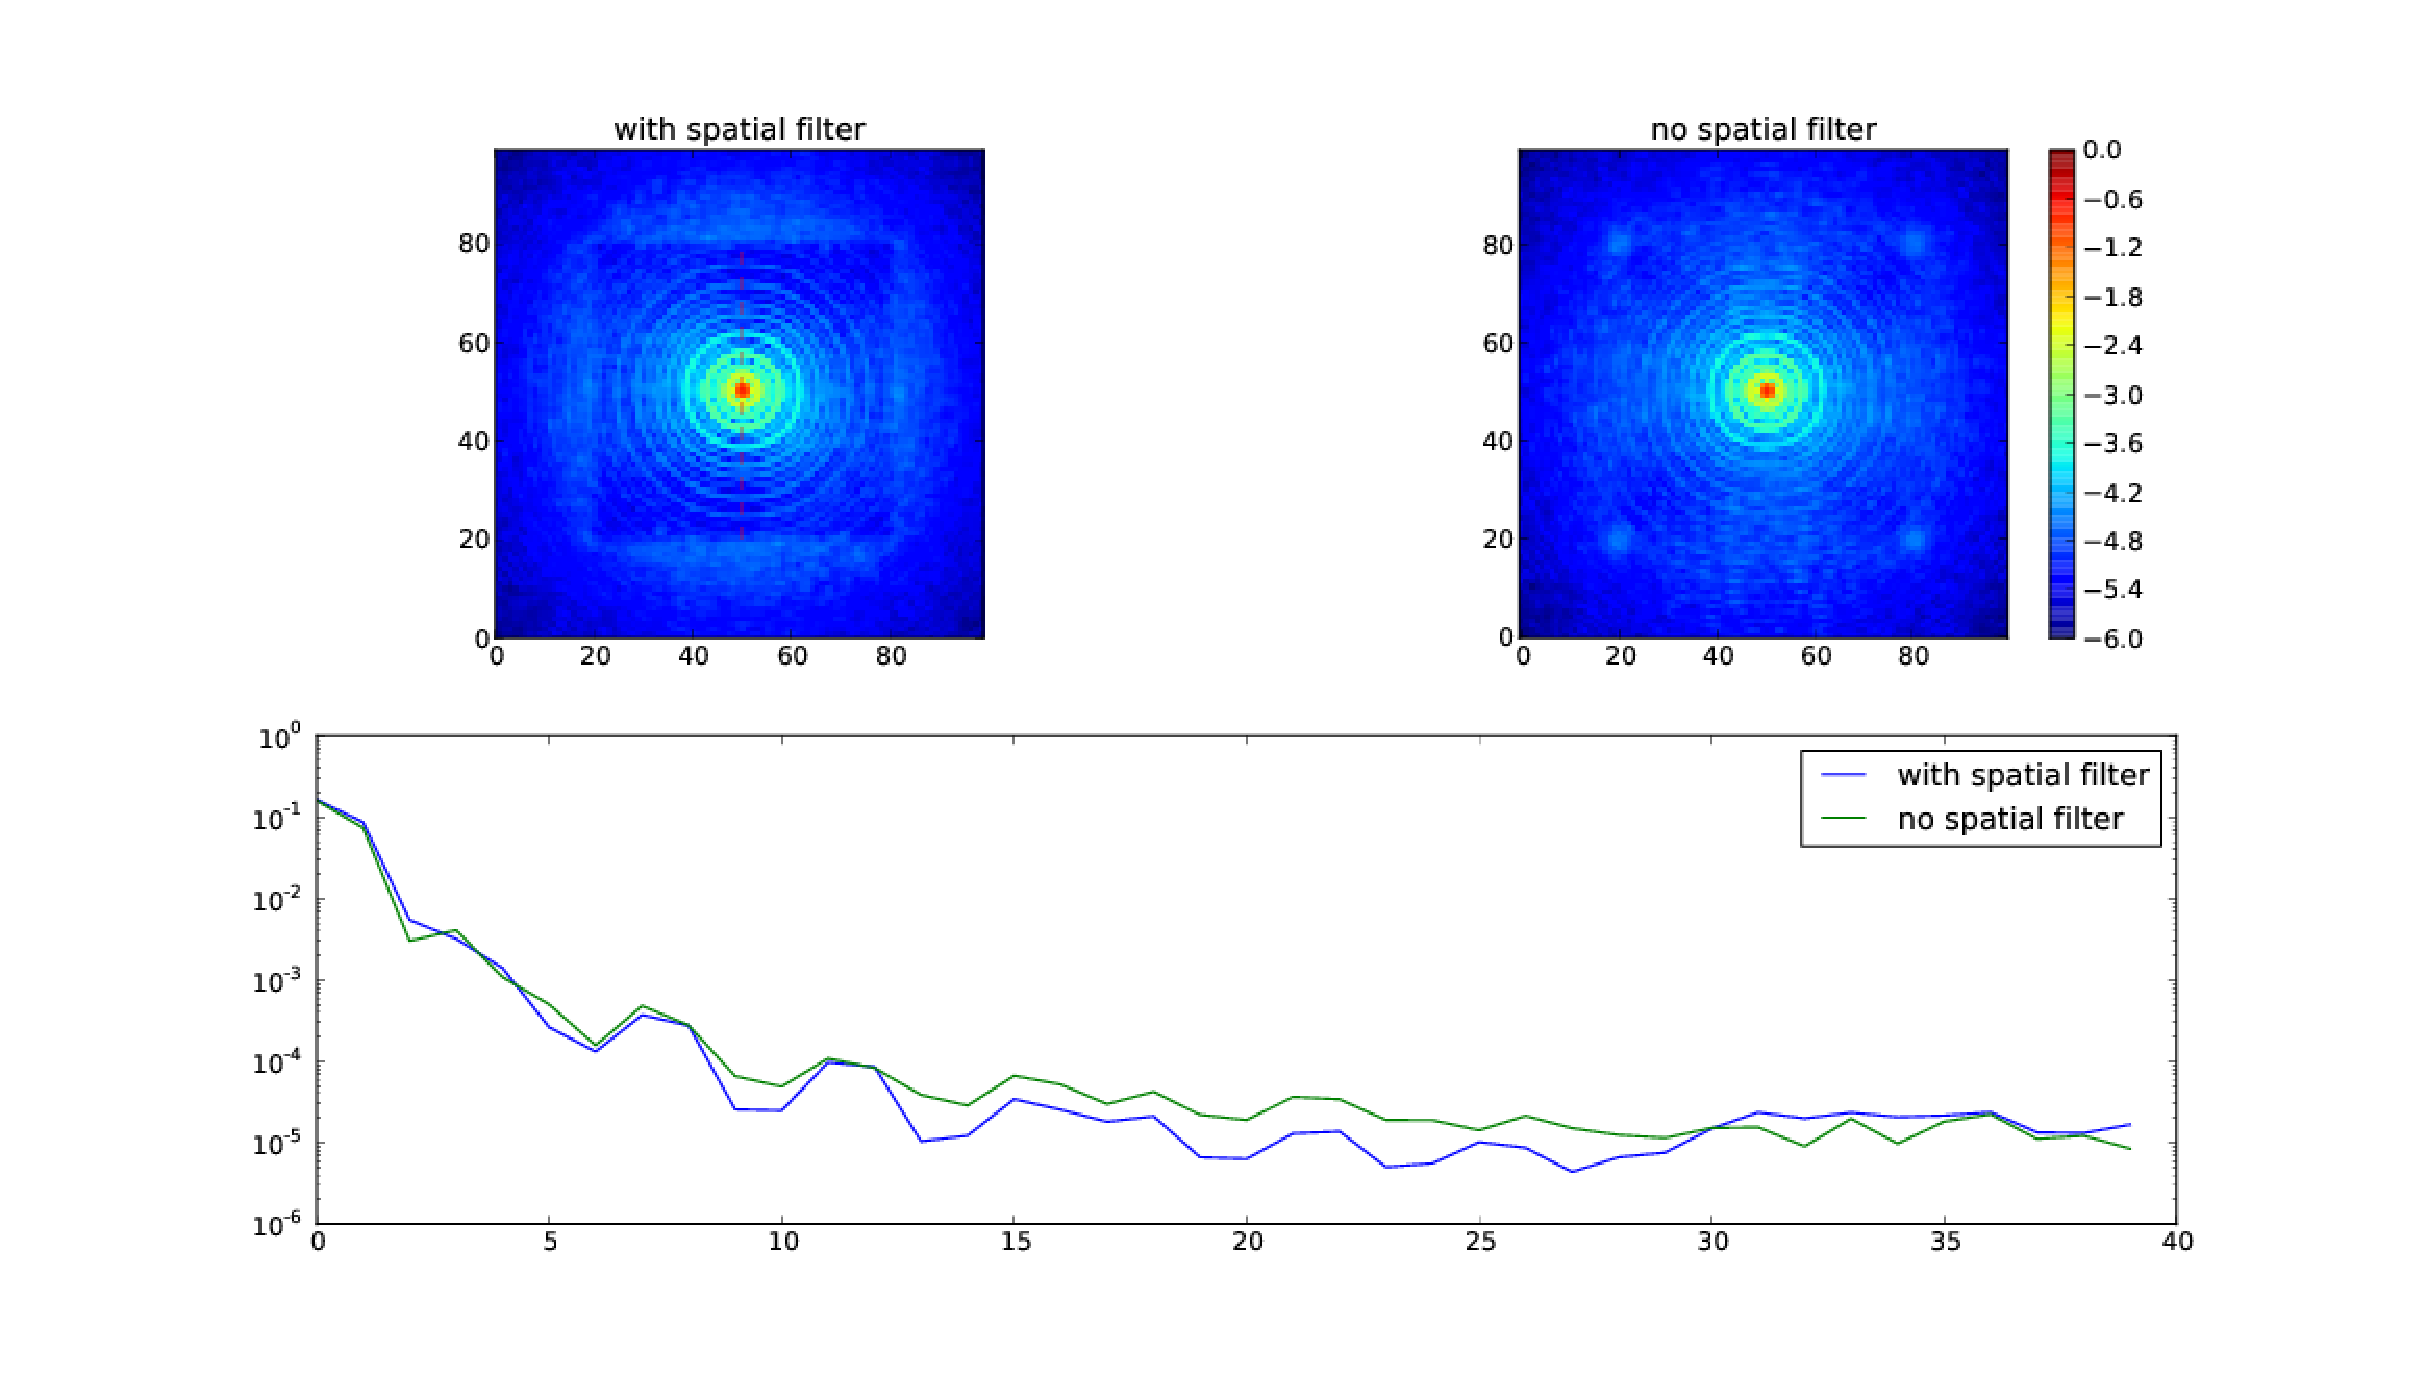
\includegraphics[width=20cm]{spatial_filter_example.eps}
\end{center}
\caption{Sample PSFs from SCAO simulations with and without a WFS spatial
filter. \label{fig:sfexamp1}}
\end{figure}

\printindex
\end{document}
